\documentclass[12pt]{amsart}

\usepackage[english, french]{babel}
\usepackage[utf8]{inputenc}
\usepackage[left=2cm,right=2cm,top=2cm,bottom=2cm]{geometry}
\usepackage{amsmath,amsthm, amssymb,amsfonts,nicefrac}
\usepackage[all]{xy}
\usepackage{amsmath}
\usepackage{graphicx}
\usepackage{textcomp}
\usepackage{color}
\usepackage{graphpap}
\usepackage[ colorlinks, linktocpage, citecolor = black, linkcolor = black]{hyperref}
\usepackage{enumitem}
\usepackage{enumerate}
\usepackage{eurosym}


\title[]{Financement}

%\address{Susanna Zimmermann\\
%Universit\'e d'Angers}
%\email{zimmermann@math.univ-angers.fr}

%%%% new list %%%
\newlist{erel}{enumerate}{1}
\setlist[erel,1]{label={\bfseries (rel. \arabic*)}}
%%%%%%%%%%%%%%%

%%% letters %%%
\newcommand{\N}{\ensuremath{\mathbb{N}}}
\newcommand{\Z}{\ensuremath{\mathbb{Z}}}
\newcommand{\Q}{\ensuremath{\mathbb{Q}}}
\newcommand{\F}{\ensuremath{\mathbb{F}}}
\newcommand{\K}{\ensuremath{\mathbb{K}}}
\newcommand{\R}{\ensuremath{\mathbb{R}}}
\newcommand{\C}{\ensuremath{\mathbb{C}}}
\newcommand{\A}{\ensuremath{\mathbb{A}}}
\newcommand{\p}{\ensuremath{\mathbb{P}}}
\newcommand{\h}{\ensuremath{\mathbb{H}}}
\renewcommand\k{\mathrm{k}}
\DeclareMathOperator{\Aut}{Aut}
\DeclareMathOperator{\End}{End}
\DeclareMathOperator{\Iso}{Iso}
\DeclareMathOperator{\GL}{GL}
\DeclareMathOperator{\SL}{SL}
\DeclareMathOperator{\Id}{Id}
\DeclareMathOperator{\Ordn}{\rm Ordn}
\DeclareMathOperator{\Frac}{Frac}
\DeclareMathOperator{\Diff}{Diff}

%%% anneaux %%%
\newcommand{\mmod}{/\!\!/}

%%% arrows %%%
\newcommand\mapsfrom{\mathrel{\reflectbox{\ensuremath{\longmapsto}}}}
\def\dashmapsto{\mapstochar\dashrightarrow}
\newcommand{\testleftlong}{\longleftarrow\!\shortmid}

%%% scale inkscape %%%
\newcommand\SB[1][\scalebox{0.6}]{#1}
\newcommand\SBa[1][\scalebox{0.8}]{#1}
\newcommand\SBb[1][\scalebox{0.9}]{#1}

%%% layout %%%
\frenchspacing
\def\lineheight{2.5mm}
%\linespread{1.2}



\begin{document}

\thispagestyle{empty}
%{\flushleft CNRS}\\

\noindent\begin{minipage}[h]{.8\textwidth}
\leftline{Susanna Zimmermann}
\leftline{Maître de Conférence}
\leftline{Laboratoire Angevin de REcherche en MAth\'ematiques }
\leftline{Universit\'e d'Angers}
\leftline{2, boulevard Lavoisier, 49045 Angers cedex 01, France }
\leftline{t\'el: 02 41 73 50 71 }
\leftline{\tt susanna.zimmermann@univ-angers.fr}
\end{minipage}
\begin{minipage}[h]{.2\textwidth}
 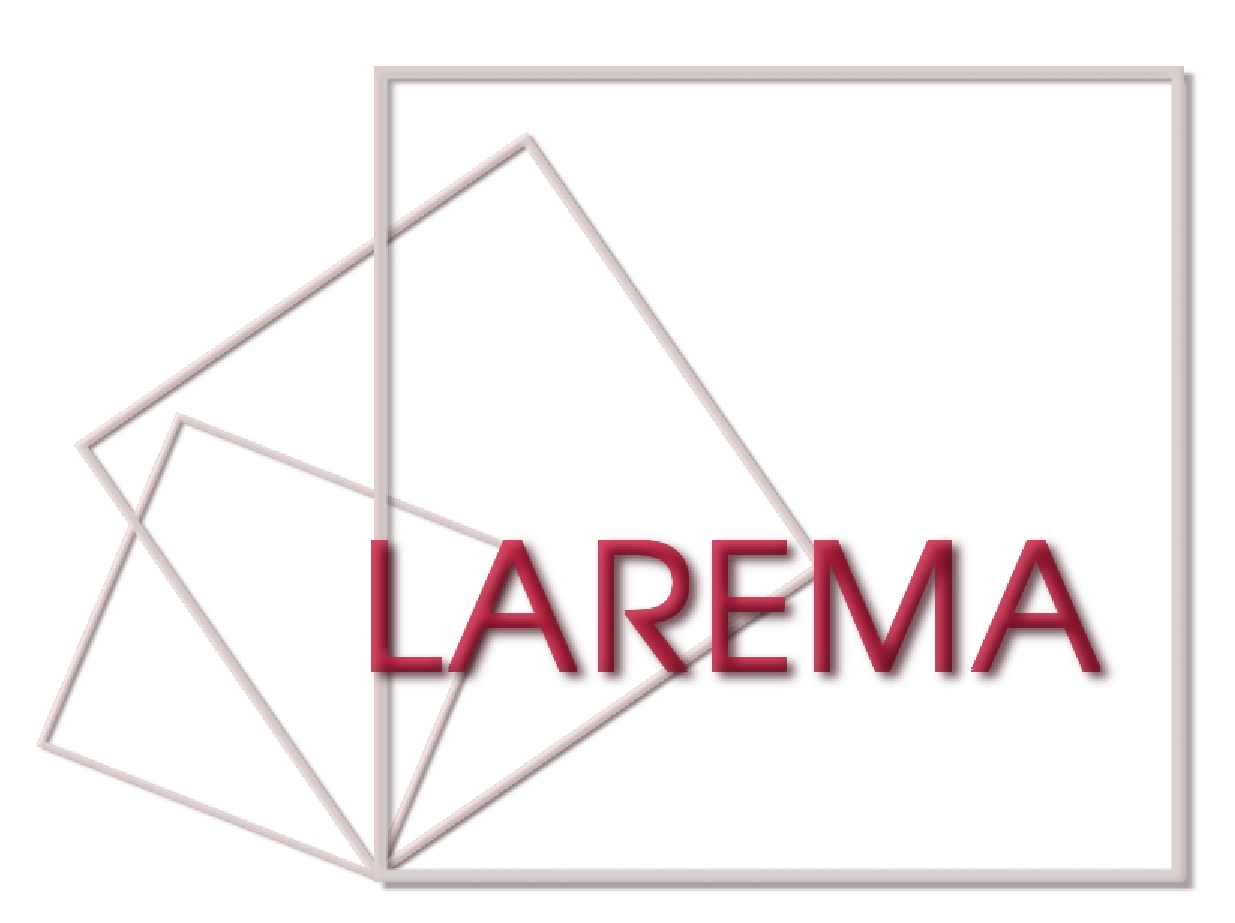
\includegraphics[scale=.14]{laremaLogoFloating}
 \includegraphics[scale=.45]{ua_h_couleur.png}
\end{minipage}
%\smallskip
%\vskip\baselineskip
%\bigskip
\vspace{1cm}

\noindent 14 julliet 2021, Angers\\[3pt]%\bigskip%\vspace{-.5cm}

\noindent{\bf Journées de GAGC à Angers, 24-26 novembre 2021}%\bigskip
\\[-3pt]

\noindent Chère madame, cher monsieur,\smallskip

Au nom de l'organisation des {\em Journées GAGC à Angers}, je souhaite demander l'autorisation que elles puissent prendre place les 24-26 novembre à la Faculté des Sciences, sous reserve que la situation sanitaire et les restriction mises en place à l'Université d'Angers le permettent. \smallskip


 Cordialement, \\
Susanna Zimmermann\vspace{1.2cm}%\vskip\baselineskip




\noindent\begin{tabular}{ l l }
Date \& endroit: & 24-26 novembre 2021, Université d'Angers\\
&24 novembre, 14-18h; 25 novembre, 9-18h; 26 novembre, 9-13h\\[6pt]
Organisation: & Stéphane Druel (Univ. Lyon 1) \\ 
&Susanna Zimmermann (Univ. d'Angers)\\[6pt] 
Comité scientifique: &  Sébastien Boucksom (CMLS, Palaiseau) \\
&Damien Calaque (Univ. Montpellier)\\
& Antoine Chambert-Loir (Univ. Paris-Diderot)\\
& Andreas Höring (Univ. de Nice Sophia-Antipolis)\\
&Laurent Manivel (Univ. Toulouse)\\
& Anne Moreau (Univ. Paris-Sud)\\ 
&Christophe Mourougane (Univ. de Rennes I) \\
&Alessandra Sarti (Univ. Poitiers)\\[6pt]
Thématiques: & Géométrie algébrique et géométrie complexe;\\
& elles sont les thématiques du GDR GAGC\\[6pt]
Orateurs, oratrices: 
&Hulya Arguz (Univ. Versailles)\\
&Pietro Beri (Univ. Toulouse)\\
& Ana-Maria Castravet (Univ. Versailles), à confirmer\\
&Benoit Claudon (Univ. Rennes)\\
&Clément Dupont (Univ. Montpellier)\\
&Antoine Etesse (Univ. Marseille)\\
&Enrica Floris (Univ. Poitiers)\\
&Julien Grivaux (Sorbonne Univ.)\\
&Mercedes Haiech (Univ. Rennes)\\
&Lucy Moser-Jauslin (Univ. Bourgogne), à confirmer\\[6pt]
No. des présent.e.s:& 35 (incl. orateurs, oratrices, organisation, participant.e.s)
\end{tabular}


\end{document}